\documentclass[border=3pt]{standalone}
\usepackage{tikz}
\usetikzlibrary{calc}
% \field{row-y}{x0}{x1}{label}
\newcommand{\field}[4]{\draw[thick] (#2,#1) rectangle (#3,#1+7);
  \node[font=\sffamily\footnotesize] at ({(#2+#3)/2},#1+3.5) {#4};}
\begin{document}
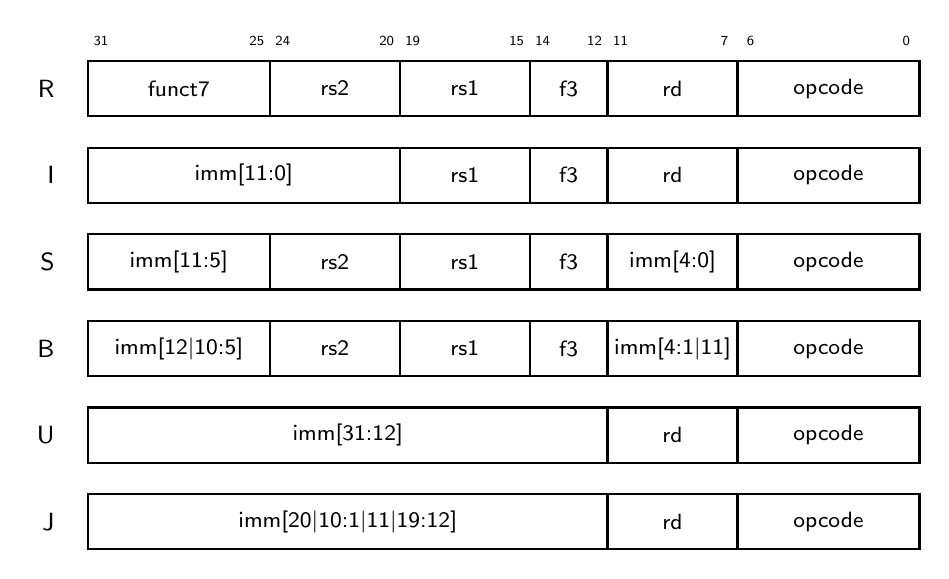
\begin{tikzpicture}[font=\sffamily\small, x=1mm, y=1mm]
  % bit ruler (w = 3.3mm/bit): bit b spans x=(31-b)*3.3 .. (32-b)*3.3
  \foreach \b/\x in {31/0, 25/19.8, 24/23.1, 20/36.3, 19/39.6, 15/52.8, 14/56.1, 12/62.7, 11/66, 7/79.2, 6/82.5, 0/102.3}{
    \node[font=\sffamily\tiny] at (\x+1.65,64.5) {\b};}
  % R-type  y=55
  \node[anchor=east] at (-3,58.5) {R};
  \field{55}{0}{23.1}{funct7}\field{55}{23.1}{39.6}{rs2}\field{55}{39.6}{56.1}{rs1}\field{55}{56.1}{66}{f3}\field{55}{66}{82.5}{rd}\field{55}{82.5}{105.6}{opcode}
  % I-type  y=44
  \node[anchor=east] at (-3,47.5) {I};
  \field{44}{0}{39.6}{imm[11:0]}\field{44}{39.6}{56.1}{rs1}\field{44}{56.1}{66}{f3}\field{44}{66}{82.5}{rd}\field{44}{82.5}{105.6}{opcode}
  % S-type  y=33
  \node[anchor=east] at (-3,36.5) {S};
  \field{33}{0}{23.1}{imm[11:5]}\field{33}{23.1}{39.6}{rs2}\field{33}{39.6}{56.1}{rs1}\field{33}{56.1}{66}{f3}\field{33}{66}{82.5}{imm[4:0]}\field{33}{82.5}{105.6}{opcode}
  % B-type  y=22
  \node[anchor=east] at (-3,25.5) {B};
  \field{22}{0}{23.1}{imm[12$|$10:5]}\field{22}{23.1}{39.6}{rs2}\field{22}{39.6}{56.1}{rs1}\field{22}{56.1}{66}{f3}\field{22}{66}{82.5}{imm[4:1$|$11]}\field{22}{82.5}{105.6}{opcode}
  % U-type  y=11
  \node[anchor=east] at (-3,14.5) {U};
  \field{11}{0}{66}{imm[31:12]}\field{11}{66}{82.5}{rd}\field{11}{82.5}{105.6}{opcode}
  % J-type  y=0
  \node[anchor=east] at (-3,3.5) {J};
  \field{0}{0}{66}{imm[20$|$10:1$|$11$|$19:12]}\field{0}{66}{82.5}{rd}\field{0}{82.5}{105.6}{opcode}
\end{tikzpicture}
\end{document}
